\section{mr::vec\_\-base$<$ C, T $>$ Struct Template Reference}
\label{structmr_1_1vec__base}\index{mr::vec_base@{mr::vec\_\-base}}
{\tt \#include $<$mr\-Vector.h$>$}

Inheritance diagram for mr::vec\_\-base$<$ C, T $>$::\begin{figure}[H]
\begin{center}
\leavevmode
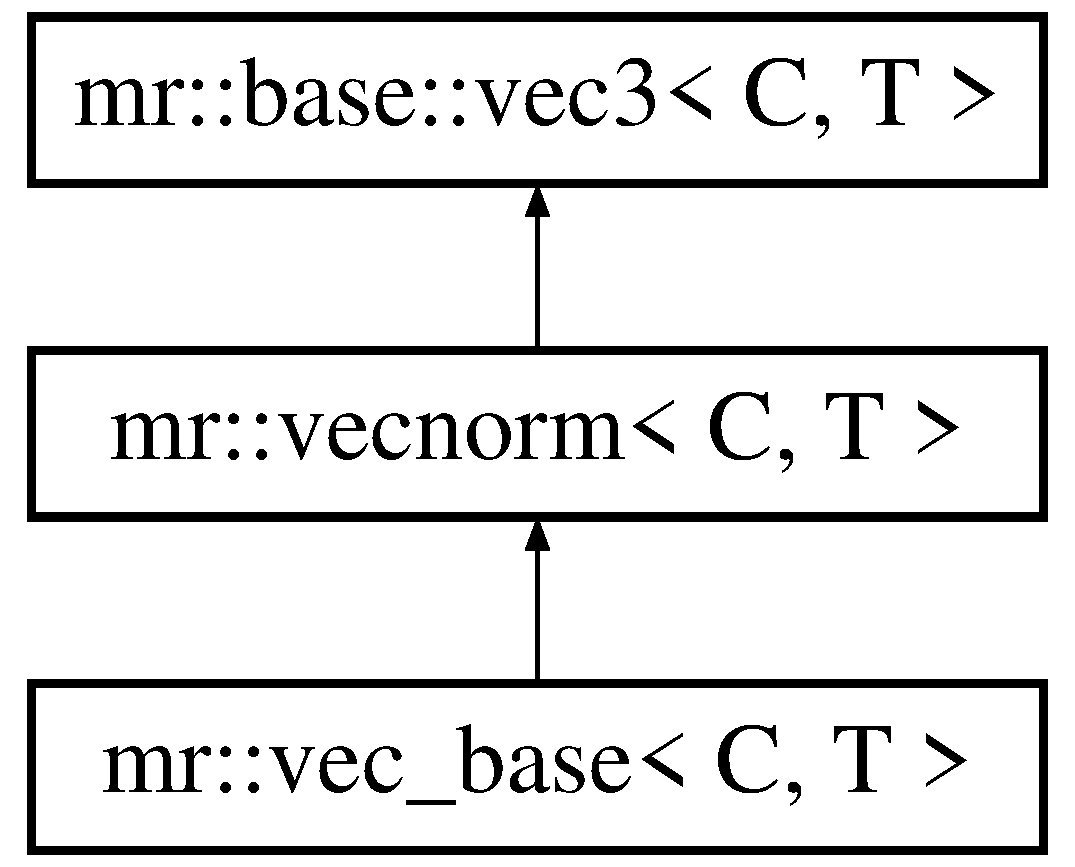
\includegraphics[height=3cm]{structmr_1_1vec__base}
\end{center}
\end{figure}
\subsection*{Public Types}
\begin{CompactItemize}
\item 
typedef {\bf vec\_\-base}$<$ C, T $>$ {\bf self}
\end{CompactItemize}
\subsection*{Public Member Functions}
\begin{CompactItemize}
\item 
void {\bf to\-Tangent} (const mi\-State $\ast$const state, const int idx=0)
\item 
void {\bf to\-Object} (const mi\-State $\ast$const state)
\item 
void {\bf to\-World} (const mi\-State $\ast$const state)
\item 
void {\bf to\-Camera} (const mi\-State $\ast$const state)
\item 
void {\bf to\-Raster} (const mi\-State $\ast$const state)
\item 
void {\bf to\-NDC} (const mi\-State $\ast$const state)
\item 
void {\bf to\-Light} (const mi\-State $\ast$const state)
\item 
void {\bf from\-Tangent} (const mi\-State $\ast$const state, const int idx=0)
\item 
void {\bf from\-Object} (const mi\-State $\ast$const state)
\item 
void {\bf from\-World} (const mi\-State $\ast$const state)
\item 
void {\bf from\-Camera} (const mi\-State $\ast$const state)
\item 
void {\bf from\-Raster} (const mi\-State $\ast$const state)
\item 
void {\bf from\-Light} (const mi\-State $\ast$const state)
\item 
void {\bf to} (const mi\-State $\ast$const state, const {\bf space::type} to\-Space)
\item 
void {\bf from} (const mi\-State $\ast$const state, const {\bf space::type} from\-Space)
\item 
void {\bf transform} (const mi\-State $\ast$const state, const {\bf space::type} from\-Space, const {\bf space::type} to\-Space)
\item 
{\bf self} {\bf inverse} () const 
\item 
{\bf self} {\bf operator-} () const 
\item 
{\bf self} {\bf normalized} () const 
\item 
{\bf self} {\bf normalized\-Fast} () const 
\item 
{\bf self} {\bf operator $\ast$} (const mi\-Matrix m) const 
\item 
{\bf self} {\bf operator $\ast$} (const {\bf matrix} \&m) const 
\end{CompactItemize}
\begin{Indent}{\bf Constructors}\par
\begin{CompactItemize}
\item 
{\bf vec\_\-base} ()
\item 
template$<$class X, class Y, class Oper$>$ {\bf vec\_\-base} (const {\bf base::exp}$<$ X, Y, Oper $>$ \&e)
\item 
{\bf vec\_\-base} ({\bf k\-No\-Construct})
\begin{CompactList}\small\item\em Empty and fast constructor. x,y,z are undefined. \item\end{CompactList}\item 
{\bf vec\_\-base} (const C \&b)
\begin{CompactList}\small\item\em Constructor from a similar mi\-Vector. \item\end{CompactList}\item 
{\bf vec\_\-base} (const T b)
\begin{CompactList}\small\item\em Constructor from a single value. \item\end{CompactList}\item 
{\bf vec\_\-base} (const T xx, const T yy, const T zz)
\begin{CompactList}\small\item\em Constructor from three values. \item\end{CompactList}\item 
{\bf vec\_\-base} (const mi\-State $\ast$const state, const {\bf space::type} from\-Space, const C \&v)
\begin{CompactList}\small\item\em Constructor from another mi\-Vector, assuming it comes from a space. \item\end{CompactList}\item 
{\bf vec\_\-base} (const mi\-State $\ast$const state, const {\bf space::type} from\-Space, const T xx, const T yy, const T zz)
\begin{CompactList}\small\item\em Constructor from 3 values, assuming they are defined in some space. \item\end{CompactList}\end{CompactItemize}
\end{Indent}
\begin{Indent}{\bf Copy Constructor}\par
\begin{CompactItemize}
\item 
{\bf vec\_\-base} (const {\bf self} \&b)
\end{CompactItemize}
\end{Indent}
\begin{Indent}{\bf Assignment}\par
\begin{CompactItemize}
\item 
template$<$class X, class Y, class Oper$>$ const {\bf self} \& {\bf operator=} (const {\bf base::exp}$<$ X, Y, Oper $>$ \&e)
\begin{CompactList}\small\item\em Handle assignment when we deal with a chained operation. \item\end{CompactList}\item 
const {\bf self} \& {\bf operator=} (const {\bf self} \&b)
\begin{CompactList}\small\item\em Assignment of similar object. \item\end{CompactList}\item 
const {\bf self} \& {\bf operator=} (const C \&b)
\begin{CompactList}\small\item\em Assignemnt of base class object. \item\end{CompactList}\item 
const {\bf self} \& {\bf operator=} (const T b)
\begin{CompactList}\small\item\em Assignment of base type. \item\end{CompactList}\end{CompactItemize}
\end{Indent}
\begin{Indent}{\bf Cross product}\par
\begin{CompactItemize}
\item 
template$<$class X, class Y, class Oper$>$ const {\bf self} \& {\bf operator$^\wedge$=} (const {\bf base::exp}$<$ X, Y, Oper $>$ \&b)
\item 
const {\bf self} \& {\bf operator$^\wedge$=} (const mi\-Vector \&b)
\item 
template$<$typename X$>$ const {\bf self} \& {\bf cross} (const X \&b)
\item 
template$<$class X, class Y, class Oper$>$ {\bf self} {\bf operator$^\wedge$} (const {\bf base::exp}$<$ X, Y, Oper $>$ \&b) const 
\item 
{\bf self} {\bf operator$^\wedge$} (const mi\-Vector \&b) const 
\end{CompactItemize}
\end{Indent}
\begin{Indent}{\bf REFERENCE OPERATORS (MODIFY IN PLACE)}\par
\begin{CompactItemize}
\item 
const {\bf self} \& {\bf operator $\ast$=} (const T b)
\item 
const {\bf self} \& {\bf operator $\ast$=} (const C \&b)
\item 
const {\bf self} \& {\bf operator $\ast$=} (const mi\-Matrix a)
\item 
const {\bf self} \& {\bf operator $\ast$=} (const {\bf matrix} \&m)
\end{CompactItemize}
\end{Indent}
\subsection*{Static Public Attributes}
\begin{CompactItemize}
\item 
{\bf vec\_\-base}$<$ C, T $>$ {\bf k\-Null}
\item 
{\bf vec\_\-base}$<$ C, T $>$ {\bf k\-Axis\-X}
\item 
{\bf vec\_\-base}$<$ C, T $>$ {\bf k\-Axis\-Y}
\item 
{\bf vec\_\-base}$<$ C, T $>$ {\bf k\-Axis\-Z}
\item 
{\bf vec\_\-base}$<$ C, T $>$ {\bf k\-Unit\-Scale}
\end{CompactItemize}
\subsubsection*{template$<$class C, typename T$>$ struct mr::vec\_\-base$<$ C, T $>$}



\subsection{Member Typedef Documentation}
\index{mr::vec_base@{mr::vec\_\-base}!self@{self}}
\index{self@{self}!mr::vec_base@{mr::vec\_\-base}}
\subsubsection{\setlength{\rightskip}{0pt plus 5cm}template$<$class C, typename T$>$ typedef {\bf vec\_\-base}$<$ C, T $>$ {\bf mr::vec\_\-base}$<$ C, T $>$::{\bf self}}\label{structmr_1_1vec__base_w0}




Reimplemented from {\bf mr::vecnorm$<$ C, T $>$} {\rm (p.\,\pageref{structmr_1_1vecnorm_w0})}.

\subsection{Constructor \& Destructor Documentation}
\index{mr::vec_base@{mr::vec\_\-base}!vec_base@{vec\_\-base}}
\index{vec_base@{vec\_\-base}!mr::vec_base@{mr::vec\_\-base}}
\subsubsection{\setlength{\rightskip}{0pt plus 5cm}template$<$class C, typename T$>$ {\bf mr::vec\_\-base}$<$ C, T $>$::{\bf vec\_\-base} ()\hspace{0.3cm}{\tt  [inline]}}\label{structmr_1_1vec__base_z58_0}


\index{mr::vec_base@{mr::vec\_\-base}!vec_base@{vec\_\-base}}
\index{vec_base@{vec\_\-base}!mr::vec_base@{mr::vec\_\-base}}
\subsubsection{\setlength{\rightskip}{0pt plus 5cm}template$<$class C, typename T$>$ template$<$class X, class Y, class Oper$>$ {\bf mr::vec\_\-base}$<$ C, T $>$::{\bf vec\_\-base} (const {\bf base::exp}$<$ X, Y, Oper $>$ \& {\em e})\hspace{0.3cm}{\tt  [inline]}}\label{structmr_1_1vec__base_z58_1}


\index{mr::vec_base@{mr::vec\_\-base}!vec_base@{vec\_\-base}}
\index{vec_base@{vec\_\-base}!mr::vec_base@{mr::vec\_\-base}}
\subsubsection{\setlength{\rightskip}{0pt plus 5cm}template$<$class C, typename T$>$ {\bf mr::vec\_\-base}$<$ C, T $>$::{\bf vec\_\-base} ({\bf k\-No\-Construct})\hspace{0.3cm}{\tt  [inline]}}\label{structmr_1_1vec__base_z58_2}


Empty and fast constructor. x,y,z are undefined. 

\index{mr::vec_base@{mr::vec\_\-base}!vec_base@{vec\_\-base}}
\index{vec_base@{vec\_\-base}!mr::vec_base@{mr::vec\_\-base}}
\subsubsection{\setlength{\rightskip}{0pt plus 5cm}template$<$class C, typename T$>$ {\bf mr::vec\_\-base}$<$ C, T $>$::{\bf vec\_\-base} (const C \& {\em b})\hspace{0.3cm}{\tt  [inline]}}\label{structmr_1_1vec__base_z58_3}


Constructor from a similar mi\-Vector. 

\index{mr::vec_base@{mr::vec\_\-base}!vec_base@{vec\_\-base}}
\index{vec_base@{vec\_\-base}!mr::vec_base@{mr::vec\_\-base}}
\subsubsection{\setlength{\rightskip}{0pt plus 5cm}template$<$class C, typename T$>$ {\bf mr::vec\_\-base}$<$ C, T $>$::{\bf vec\_\-base} (const T {\em b})\hspace{0.3cm}{\tt  [inline]}}\label{structmr_1_1vec__base_z58_4}


Constructor from a single value. 

\index{mr::vec_base@{mr::vec\_\-base}!vec_base@{vec\_\-base}}
\index{vec_base@{vec\_\-base}!mr::vec_base@{mr::vec\_\-base}}
\subsubsection{\setlength{\rightskip}{0pt plus 5cm}template$<$class C, typename T$>$ {\bf mr::vec\_\-base}$<$ C, T $>$::{\bf vec\_\-base} (const T {\em xx}, const T {\em yy}, const T {\em zz})\hspace{0.3cm}{\tt  [inline]}}\label{structmr_1_1vec__base_z58_5}


Constructor from three values. 

\index{mr::vec_base@{mr::vec\_\-base}!vec_base@{vec\_\-base}}
\index{vec_base@{vec\_\-base}!mr::vec_base@{mr::vec\_\-base}}
\subsubsection{\setlength{\rightskip}{0pt plus 5cm}template$<$class C, typename T$>$ {\bf mr::vec\_\-base}$<$ C, T $>$::{\bf vec\_\-base} (const mi\-State $\ast$const {\em state}, const {\bf space::type} {\em from\-Space}, const C \& {\em v})\hspace{0.3cm}{\tt  [inline]}}\label{structmr_1_1vec__base_z58_6}


Constructor from another mi\-Vector, assuming it comes from a space. 

\index{mr::vec_base@{mr::vec\_\-base}!vec_base@{vec\_\-base}}
\index{vec_base@{vec\_\-base}!mr::vec_base@{mr::vec\_\-base}}
\subsubsection{\setlength{\rightskip}{0pt plus 5cm}template$<$class C, typename T$>$ {\bf mr::vec\_\-base}$<$ C, T $>$::{\bf vec\_\-base} (const mi\-State $\ast$const {\em state}, const {\bf space::type} {\em from\-Space}, const T {\em xx}, const T {\em yy}, const T {\em zz})\hspace{0.3cm}{\tt  [inline]}}\label{structmr_1_1vec__base_z58_7}


Constructor from 3 values, assuming they are defined in some space. 

\index{mr::vec_base@{mr::vec\_\-base}!vec_base@{vec\_\-base}}
\index{vec_base@{vec\_\-base}!mr::vec_base@{mr::vec\_\-base}}
\subsubsection{\setlength{\rightskip}{0pt plus 5cm}template$<$class C, typename T$>$ {\bf mr::vec\_\-base}$<$ C, T $>$::{\bf vec\_\-base} (const {\bf self} \& {\em b})\hspace{0.3cm}{\tt  [inline]}}\label{structmr_1_1vec__base_z59_0}




\subsection{Member Function Documentation}
\index{mr::vec_base@{mr::vec\_\-base}!cross@{cross}}
\index{cross@{cross}!mr::vec_base@{mr::vec\_\-base}}
\subsubsection{\setlength{\rightskip}{0pt plus 5cm}template$<$class C, typename T$>$ template$<$typename X$>$ const {\bf self}\& {\bf mr::vec\_\-base}$<$ C, T $>$::cross (const X \& {\em b})\hspace{0.3cm}{\tt  [inline]}}\label{structmr_1_1vec__base_z62_2}


\index{mr::vec_base@{mr::vec\_\-base}!from@{from}}
\index{from@{from}!mr::vec_base@{mr::vec\_\-base}}
\subsubsection{\setlength{\rightskip}{0pt plus 5cm}template$<$class C, typename T$>$ void {\bf mr::vec\_\-base}$<$ C, T $>$::from (const mi\-State $\ast$const {\em state}, const {\bf space::type} {\em from\-Space})\hspace{0.3cm}{\tt  [inline]}}\label{structmr_1_1vec__base_a14}


\index{mr::vec_base@{mr::vec\_\-base}!fromCamera@{fromCamera}}
\index{fromCamera@{fromCamera}!mr::vec_base@{mr::vec\_\-base}}
\subsubsection{\setlength{\rightskip}{0pt plus 5cm}template$<$class C, typename T$>$ void {\bf mr::vec\_\-base}$<$ C, T $>$::from\-Camera (const mi\-State $\ast$const {\em state})\hspace{0.3cm}{\tt  [inline]}}\label{structmr_1_1vec__base_a10}


\index{mr::vec_base@{mr::vec\_\-base}!fromLight@{fromLight}}
\index{fromLight@{fromLight}!mr::vec_base@{mr::vec\_\-base}}
\subsubsection{\setlength{\rightskip}{0pt plus 5cm}template$<$class C, typename T$>$ void {\bf mr::vec\_\-base}$<$ C, T $>$::from\-Light (const mi\-State $\ast$const {\em state})\hspace{0.3cm}{\tt  [inline]}}\label{structmr_1_1vec__base_a12}


\index{mr::vec_base@{mr::vec\_\-base}!fromObject@{fromObject}}
\index{fromObject@{fromObject}!mr::vec_base@{mr::vec\_\-base}}
\subsubsection{\setlength{\rightskip}{0pt plus 5cm}template$<$class C, typename T$>$ void {\bf mr::vec\_\-base}$<$ C, T $>$::from\-Object (const mi\-State $\ast$const {\em state})\hspace{0.3cm}{\tt  [inline]}}\label{structmr_1_1vec__base_a8}


\index{mr::vec_base@{mr::vec\_\-base}!fromRaster@{fromRaster}}
\index{fromRaster@{fromRaster}!mr::vec_base@{mr::vec\_\-base}}
\subsubsection{\setlength{\rightskip}{0pt plus 5cm}template$<$class C, typename T$>$ void {\bf mr::vec\_\-base}$<$ C, T $>$::from\-Raster (const mi\-State $\ast$const {\em state})\hspace{0.3cm}{\tt  [inline]}}\label{structmr_1_1vec__base_a11}


\index{mr::vec_base@{mr::vec\_\-base}!fromTangent@{fromTangent}}
\index{fromTangent@{fromTangent}!mr::vec_base@{mr::vec\_\-base}}
\subsubsection{\setlength{\rightskip}{0pt plus 5cm}template$<$class C, typename T$>$ void {\bf mr::vec\_\-base}$<$ C, T $>$::from\-Tangent (const mi\-State $\ast$const {\em state}, const int {\em idx} = 0)\hspace{0.3cm}{\tt  [inline]}}\label{structmr_1_1vec__base_a7}


\index{mr::vec_base@{mr::vec\_\-base}!fromWorld@{fromWorld}}
\index{fromWorld@{fromWorld}!mr::vec_base@{mr::vec\_\-base}}
\subsubsection{\setlength{\rightskip}{0pt plus 5cm}template$<$class C, typename T$>$ void {\bf mr::vec\_\-base}$<$ C, T $>$::from\-World (const mi\-State $\ast$const {\em state})\hspace{0.3cm}{\tt  [inline]}}\label{structmr_1_1vec__base_a9}


\index{mr::vec_base@{mr::vec\_\-base}!inverse@{inverse}}
\index{inverse@{inverse}!mr::vec_base@{mr::vec\_\-base}}
\subsubsection{\setlength{\rightskip}{0pt plus 5cm}template$<$class C, typename T$>$ {\bf self} {\bf mr::vec\_\-base}$<$ C, T $>$::inverse () const\hspace{0.3cm}{\tt  [inline]}}\label{structmr_1_1vec__base_a16}


\index{mr::vec_base@{mr::vec\_\-base}!normalized@{normalized}}
\index{normalized@{normalized}!mr::vec_base@{mr::vec\_\-base}}
\subsubsection{\setlength{\rightskip}{0pt plus 5cm}template$<$class C, typename T$>$ {\bf self} {\bf mr::vec\_\-base}$<$ C, T $>$::normalized () const\hspace{0.3cm}{\tt  [inline]}}\label{structmr_1_1vec__base_a18}


\index{mr::vec_base@{mr::vec\_\-base}!normalizedFast@{normalizedFast}}
\index{normalizedFast@{normalizedFast}!mr::vec_base@{mr::vec\_\-base}}
\subsubsection{\setlength{\rightskip}{0pt plus 5cm}template$<$class C, typename T$>$ {\bf self} {\bf mr::vec\_\-base}$<$ C, T $>$::normalized\-Fast () const\hspace{0.3cm}{\tt  [inline]}}\label{structmr_1_1vec__base_a19}


\index{mr::vec_base@{mr::vec\_\-base}!operator *@{operator $\ast$}}
\index{operator *@{operator $\ast$}!mr::vec_base@{mr::vec\_\-base}}
\subsubsection{\setlength{\rightskip}{0pt plus 5cm}template$<$class C, typename T$>$ {\bf self} {\bf mr::vec\_\-base}$<$ C, T $>$::operator $\ast$ (const {\bf matrix} \& {\em m}) const\hspace{0.3cm}{\tt  [inline]}}\label{structmr_1_1vec__base_a21}


\index{mr::vec_base@{mr::vec\_\-base}!operator *@{operator $\ast$}}
\index{operator *@{operator $\ast$}!mr::vec_base@{mr::vec\_\-base}}
\subsubsection{\setlength{\rightskip}{0pt plus 5cm}template$<$class C, typename T$>$ {\bf self} {\bf mr::vec\_\-base}$<$ C, T $>$::operator $\ast$ (const mi\-Matrix {\em m}) const\hspace{0.3cm}{\tt  [inline]}}\label{structmr_1_1vec__base_a20}


\index{mr::vec_base@{mr::vec\_\-base}!operator *=@{operator $\ast$=}}
\index{operator *=@{operator $\ast$=}!mr::vec_base@{mr::vec\_\-base}}
\subsubsection{\setlength{\rightskip}{0pt plus 5cm}template$<$class C, typename T$>$ const {\bf self}\& {\bf mr::vec\_\-base}$<$ C, T $>$::operator $\ast$= (const {\bf matrix} \& {\em m})\hspace{0.3cm}{\tt  [inline]}}\label{structmr_1_1vec__base_z64_3}


\index{mr::vec_base@{mr::vec\_\-base}!operator *=@{operator $\ast$=}}
\index{operator *=@{operator $\ast$=}!mr::vec_base@{mr::vec\_\-base}}
\subsubsection{\setlength{\rightskip}{0pt plus 5cm}template$<$class C, typename T$>$ const {\bf self}\& {\bf mr::vec\_\-base}$<$ C, T $>$::operator $\ast$= (const mi\-Matrix {\em a})\hspace{0.3cm}{\tt  [inline]}}\label{structmr_1_1vec__base_z64_2}


\index{mr::vec_base@{mr::vec\_\-base}!operator *=@{operator $\ast$=}}
\index{operator *=@{operator $\ast$=}!mr::vec_base@{mr::vec\_\-base}}
\subsubsection{\setlength{\rightskip}{0pt plus 5cm}template$<$class C, typename T$>$ const {\bf self}\& {\bf mr::vec\_\-base}$<$ C, T $>$::operator $\ast$= (const C \& {\em b})\hspace{0.3cm}{\tt  [inline]}}\label{structmr_1_1vec__base_z64_1}




Reimplemented from {\bf mr::base::vec3$<$ C, T $>$} {\rm (p.\,\pageref{structmr_1_1base_1_1vec3_z40_8})}.\index{mr::vec_base@{mr::vec\_\-base}!operator *=@{operator $\ast$=}}
\index{operator *=@{operator $\ast$=}!mr::vec_base@{mr::vec\_\-base}}
\subsubsection{\setlength{\rightskip}{0pt plus 5cm}template$<$class C, typename T$>$ const {\bf self}\& {\bf mr::vec\_\-base}$<$ C, T $>$::operator $\ast$= (const T {\em b})\hspace{0.3cm}{\tt  [inline]}}\label{structmr_1_1vec__base_z64_0}




Reimplemented from {\bf mr::base::vec3$<$ C, T $>$} {\rm (p.\,\pageref{structmr_1_1base_1_1vec3_z40_7})}.\index{mr::vec_base@{mr::vec\_\-base}!operator-@{operator-}}
\index{operator-@{operator-}!mr::vec_base@{mr::vec\_\-base}}
\subsubsection{\setlength{\rightskip}{0pt plus 5cm}template$<$class C, typename T$>$ {\bf self} {\bf mr::vec\_\-base}$<$ C, T $>$::operator- () const\hspace{0.3cm}{\tt  [inline]}}\label{structmr_1_1vec__base_a17}


\index{mr::vec_base@{mr::vec\_\-base}!operator=@{operator=}}
\index{operator=@{operator=}!mr::vec_base@{mr::vec\_\-base}}
\subsubsection{\setlength{\rightskip}{0pt plus 5cm}template$<$class C, typename T$>$ const {\bf self}\& {\bf mr::vec\_\-base}$<$ C, T $>$::operator= (const T {\em b})\hspace{0.3cm}{\tt  [inline]}}\label{structmr_1_1vec__base_z60_3}


Assignment of base type. 



Reimplemented from {\bf mr::base::vec3$<$ C, T $>$} {\rm (p.\,\pageref{structmr_1_1base_1_1vec3_z36_3})}.\index{mr::vec_base@{mr::vec\_\-base}!operator=@{operator=}}
\index{operator=@{operator=}!mr::vec_base@{mr::vec\_\-base}}
\subsubsection{\setlength{\rightskip}{0pt plus 5cm}template$<$class C, typename T$>$ const {\bf self}\& {\bf mr::vec\_\-base}$<$ C, T $>$::operator= (const C \& {\em b})\hspace{0.3cm}{\tt  [inline]}}\label{structmr_1_1vec__base_z60_2}


Assignemnt of base class object. 



Reimplemented from {\bf mr::base::vec3$<$ C, T $>$} {\rm (p.\,\pageref{structmr_1_1base_1_1vec3_z36_2})}.\index{mr::vec_base@{mr::vec\_\-base}!operator=@{operator=}}
\index{operator=@{operator=}!mr::vec_base@{mr::vec\_\-base}}
\subsubsection{\setlength{\rightskip}{0pt plus 5cm}template$<$class C, typename T$>$ const {\bf self}\& {\bf mr::vec\_\-base}$<$ C, T $>$::operator= (const {\bf self} \& {\em b})\hspace{0.3cm}{\tt  [inline]}}\label{structmr_1_1vec__base_z60_1}


Assignment of similar object. 



Reimplemented from {\bf mr::base::vec3$<$ C, T $>$} {\rm (p.\,\pageref{structmr_1_1base_1_1vec3_z36_1})}.\index{mr::vec_base@{mr::vec\_\-base}!operator=@{operator=}}
\index{operator=@{operator=}!mr::vec_base@{mr::vec\_\-base}}
\subsubsection{\setlength{\rightskip}{0pt plus 5cm}template$<$class C, typename T$>$ template$<$class X, class Y, class Oper$>$ const {\bf self}\& {\bf mr::vec\_\-base}$<$ C, T $>$::operator= (const {\bf base::exp}$<$ X, Y, Oper $>$ \& {\em e})\hspace{0.3cm}{\tt  [inline]}}\label{structmr_1_1vec__base_z60_0}


Handle assignment when we deal with a chained operation. 



Reimplemented from {\bf mr::base::vec3$<$ C, T $>$} {\rm (p.\,\pageref{structmr_1_1base_1_1vec3_z36_0})}.\index{mr::vec_base@{mr::vec\_\-base}!operator^@{operator$^\wedge$}}
\index{operator^@{operator$^\wedge$}!mr::vec_base@{mr::vec\_\-base}}
\subsubsection{\setlength{\rightskip}{0pt plus 5cm}template$<$class C, typename T$>$ {\bf self} {\bf mr::vec\_\-base}$<$ C, T $>$::operator$^\wedge$ (const mi\-Vector \& {\em b}) const\hspace{0.3cm}{\tt  [inline]}}\label{structmr_1_1vec__base_z62_4}


\index{mr::vec_base@{mr::vec\_\-base}!operator^@{operator$^\wedge$}}
\index{operator^@{operator$^\wedge$}!mr::vec_base@{mr::vec\_\-base}}
\subsubsection{\setlength{\rightskip}{0pt plus 5cm}template$<$class C, typename T$>$ template$<$class X, class Y, class Oper$>$ {\bf self} {\bf mr::vec\_\-base}$<$ C, T $>$::operator$^\wedge$ (const {\bf base::exp}$<$ X, Y, Oper $>$ \& {\em b}) const\hspace{0.3cm}{\tt  [inline]}}\label{structmr_1_1vec__base_z62_3}


\index{mr::vec_base@{mr::vec\_\-base}!operator^=@{operator$^\wedge$=}}
\index{operator^=@{operator$^\wedge$=}!mr::vec_base@{mr::vec\_\-base}}
\subsubsection{\setlength{\rightskip}{0pt plus 5cm}template$<$class C, typename T$>$ const {\bf self}\& {\bf mr::vec\_\-base}$<$ C, T $>$::operator$^\wedge$= (const mi\-Vector \& {\em b})\hspace{0.3cm}{\tt  [inline]}}\label{structmr_1_1vec__base_z62_1}


\index{mr::vec_base@{mr::vec\_\-base}!operator^=@{operator$^\wedge$=}}
\index{operator^=@{operator$^\wedge$=}!mr::vec_base@{mr::vec\_\-base}}
\subsubsection{\setlength{\rightskip}{0pt plus 5cm}template$<$class C, typename T$>$ template$<$class X, class Y, class Oper$>$ const {\bf self}\& {\bf mr::vec\_\-base}$<$ C, T $>$::operator$^\wedge$= (const {\bf base::exp}$<$ X, Y, Oper $>$ \& {\em b})\hspace{0.3cm}{\tt  [inline]}}\label{structmr_1_1vec__base_z62_0}


\index{mr::vec_base@{mr::vec\_\-base}!to@{to}}
\index{to@{to}!mr::vec_base@{mr::vec\_\-base}}
\subsubsection{\setlength{\rightskip}{0pt plus 5cm}template$<$class C, typename T$>$ void {\bf mr::vec\_\-base}$<$ C, T $>$::to (const mi\-State $\ast$const {\em state}, const {\bf space::type} {\em to\-Space})\hspace{0.3cm}{\tt  [inline]}}\label{structmr_1_1vec__base_a13}


\index{mr::vec_base@{mr::vec\_\-base}!toCamera@{toCamera}}
\index{toCamera@{toCamera}!mr::vec_base@{mr::vec\_\-base}}
\subsubsection{\setlength{\rightskip}{0pt plus 5cm}template$<$class C, typename T$>$ void {\bf mr::vec\_\-base}$<$ C, T $>$::to\-Camera (const mi\-State $\ast$const {\em state})\hspace{0.3cm}{\tt  [inline]}}\label{structmr_1_1vec__base_a3}


\index{mr::vec_base@{mr::vec\_\-base}!toLight@{toLight}}
\index{toLight@{toLight}!mr::vec_base@{mr::vec\_\-base}}
\subsubsection{\setlength{\rightskip}{0pt plus 5cm}template$<$class C, typename T$>$ void {\bf mr::vec\_\-base}$<$ C, T $>$::to\-Light (const mi\-State $\ast$const {\em state})\hspace{0.3cm}{\tt  [inline]}}\label{structmr_1_1vec__base_a6}


\index{mr::vec_base@{mr::vec\_\-base}!toNDC@{toNDC}}
\index{toNDC@{toNDC}!mr::vec_base@{mr::vec\_\-base}}
\subsubsection{\setlength{\rightskip}{0pt plus 5cm}template$<$class C, typename T$>$ void {\bf mr::vec\_\-base}$<$ C, T $>$::to\-NDC (const mi\-State $\ast$const {\em state})\hspace{0.3cm}{\tt  [inline]}}\label{structmr_1_1vec__base_a5}


\index{mr::vec_base@{mr::vec\_\-base}!toObject@{toObject}}
\index{toObject@{toObject}!mr::vec_base@{mr::vec\_\-base}}
\subsubsection{\setlength{\rightskip}{0pt plus 5cm}template$<$class C, typename T$>$ void {\bf mr::vec\_\-base}$<$ C, T $>$::to\-Object (const mi\-State $\ast$const {\em state})\hspace{0.3cm}{\tt  [inline]}}\label{structmr_1_1vec__base_a1}


\index{mr::vec_base@{mr::vec\_\-base}!toRaster@{toRaster}}
\index{toRaster@{toRaster}!mr::vec_base@{mr::vec\_\-base}}
\subsubsection{\setlength{\rightskip}{0pt plus 5cm}template$<$class C, typename T$>$ void {\bf mr::vec\_\-base}$<$ C, T $>$::to\-Raster (const mi\-State $\ast$const {\em state})\hspace{0.3cm}{\tt  [inline]}}\label{structmr_1_1vec__base_a4}


\index{mr::vec_base@{mr::vec\_\-base}!toTangent@{toTangent}}
\index{toTangent@{toTangent}!mr::vec_base@{mr::vec\_\-base}}
\subsubsection{\setlength{\rightskip}{0pt plus 5cm}template$<$class C, typename T$>$ void {\bf mr::vec\_\-base}$<$ C, T $>$::to\-Tangent (const mi\-State $\ast$const {\em state}, const int {\em idx} = 0)\hspace{0.3cm}{\tt  [inline]}}\label{structmr_1_1vec__base_a0}


\index{mr::vec_base@{mr::vec\_\-base}!toWorld@{toWorld}}
\index{toWorld@{toWorld}!mr::vec_base@{mr::vec\_\-base}}
\subsubsection{\setlength{\rightskip}{0pt plus 5cm}template$<$class C, typename T$>$ void {\bf mr::vec\_\-base}$<$ C, T $>$::to\-World (const mi\-State $\ast$const {\em state})\hspace{0.3cm}{\tt  [inline]}}\label{structmr_1_1vec__base_a2}


\index{mr::vec_base@{mr::vec\_\-base}!transform@{transform}}
\index{transform@{transform}!mr::vec_base@{mr::vec\_\-base}}
\subsubsection{\setlength{\rightskip}{0pt plus 5cm}template$<$class C, typename T$>$ void {\bf mr::vec\_\-base}$<$ C, T $>$::transform (const mi\-State $\ast$const {\em state}, const {\bf space::type} {\em from\-Space}, const {\bf space::type} {\em to\-Space})\hspace{0.3cm}{\tt  [inline]}}\label{structmr_1_1vec__base_a15}




\subsection{Member Data Documentation}
\index{mr::vec_base@{mr::vec\_\-base}!kAxisX@{kAxisX}}
\index{kAxisX@{kAxisX}!mr::vec_base@{mr::vec\_\-base}}
\subsubsection{\setlength{\rightskip}{0pt plus 5cm}template$<$class C, typename T$>$ {\bf vec\_\-base}$<$ C, T $>$ {\bf mr::vec\_\-base}$<$ C, T $>$::{\bf k\-Axis\-X}\hspace{0.3cm}{\tt  [static]}}\label{structmr_1_1vec__base_s1}


\index{mr::vec_base@{mr::vec\_\-base}!kAxisY@{kAxisY}}
\index{kAxisY@{kAxisY}!mr::vec_base@{mr::vec\_\-base}}
\subsubsection{\setlength{\rightskip}{0pt plus 5cm}template$<$class C, typename T$>$ {\bf vec\_\-base}$<$ C, T $>$ {\bf mr::vec\_\-base}$<$ C, T $>$::{\bf k\-Axis\-Y}\hspace{0.3cm}{\tt  [static]}}\label{structmr_1_1vec__base_s2}


\index{mr::vec_base@{mr::vec\_\-base}!kAxisZ@{kAxisZ}}
\index{kAxisZ@{kAxisZ}!mr::vec_base@{mr::vec\_\-base}}
\subsubsection{\setlength{\rightskip}{0pt plus 5cm}template$<$class C, typename T$>$ {\bf vec\_\-base}$<$ C, T $>$ {\bf mr::vec\_\-base}$<$ C, T $>$::{\bf k\-Axis\-Z}\hspace{0.3cm}{\tt  [static]}}\label{structmr_1_1vec__base_s3}


\index{mr::vec_base@{mr::vec\_\-base}!kNull@{kNull}}
\index{kNull@{kNull}!mr::vec_base@{mr::vec\_\-base}}
\subsubsection{\setlength{\rightskip}{0pt plus 5cm}template$<$class C, typename T$>$ {\bf vec\_\-base}$<$ C, T $>$ {\bf mr::vec\_\-base}$<$ C, T $>$::{\bf k\-Null}\hspace{0.3cm}{\tt  [static]}}\label{structmr_1_1vec__base_s0}


\index{mr::vec_base@{mr::vec\_\-base}!kUnitScale@{kUnitScale}}
\index{kUnitScale@{kUnitScale}!mr::vec_base@{mr::vec\_\-base}}
\subsubsection{\setlength{\rightskip}{0pt plus 5cm}template$<$class C, typename T$>$ {\bf vec\_\-base}$<$ C, T $>$ {\bf mr::vec\_\-base}$<$ C, T $>$::{\bf k\-Unit\-Scale}\hspace{0.3cm}{\tt  [static]}}\label{structmr_1_1vec__base_s4}




The documentation for this struct was generated from the following files:\begin{CompactItemize}
\item 
{\bf mr\-Vector.h}\item 
{\bf mr\-Derivs.h}\end{CompactItemize}
